\chapter{Elementarne wiadomości o sieciach neuronowych}

W ciągu ostatnich dekad obserwuje się rozwój badań nad sztucznymi sieciami neuronowymi. Badania te są prowadzone przez naukowców z różnych dziedzin, a ich rozwój jest motywowany osiągnięciami w zakresie badania mózgu człowieka. Obecnie odkryto wiele tajemnic działania mózgu. Wiadomo na przykład jaka jest budowa komórek nerwowych (neuronów) albo w jaki sposób wymieniają one informacje między sobą \citep[s. 13]{Kosinski2017}.

Pomimo długich badań fundamentalne pytania o samą istotę działania mózgu nadal pozostają w mocy. Ciągle nie potrafimy jednoznacznie ustalić czym jest myśl ludzka albo rozwiązać  zagadkę istnienia świadomości. Fascynujące są dla nas także możliwości mózgu -- jego niezwykła zdolność do nauki i adaptacji do otoczenia oraz umiejętność myślenia kreatywnego i tworzenia nowych rzeczy \citep[s. 14]{Kosinski2017}.

Z inżynieryjnego punktu widzenia stworzenie inteligentnych układów powinno się opłacić, ponieważ maszyna byłaby zdolna wyręczyć człowieka w wykonywaniu różnych skomplikowanych prac. Powstanie \textit{sztucznych sieci neuronowych} było krokiem naprzód w realizacji tego przedsięwzięcia. Sieci takie mają niektóre właściwości mózgu człowieka. Posiadają zarówno zdolność do generalizacji (czyli do uogólniania nabytej wiedzy na nowe, nieznane przypadki), oraz zdolność do rozwiązywania zadań nieprecyzyjnie zdefiniowanych formalnie. Sieci takie mogą działać nawet przy pewnym poziomie uszkodzeń. Mają także stosunkowo duża prędkość przetwarzania informacji \citep[s. 15-16]{Kosinski2017}.

Sztuczne sieci neuronowe mogą być realizowane na dwa sposoby. W postaci sprzętowej sieć jest specjalnie zaprojektowanym układem scalonym. Zaprojektowanie układu scalonego jest kosztowne, zatem stosuje się taką implementacje tylko dla modeli, których działanie zostało wcześniej potwierdzone. (zob. rys. 1) Innym rozwiązaniem jest realizacja sieci jako programu komputerowego. Jest to implementacja posiadająca dużą elastyczność, bardzo łatwo jest dokonać zmian w~architekturze samej sieci. Dlatego tez programy komputerowe wykorzystuje się głównie na etapie badań samego modelu sieci, kiedy skuteczność końcowa modelu nie została dokładnie zbadana i udowodniona \citep[s. 15]{Kosinski2017}.

\begin{figure}[H]
\begin{center}
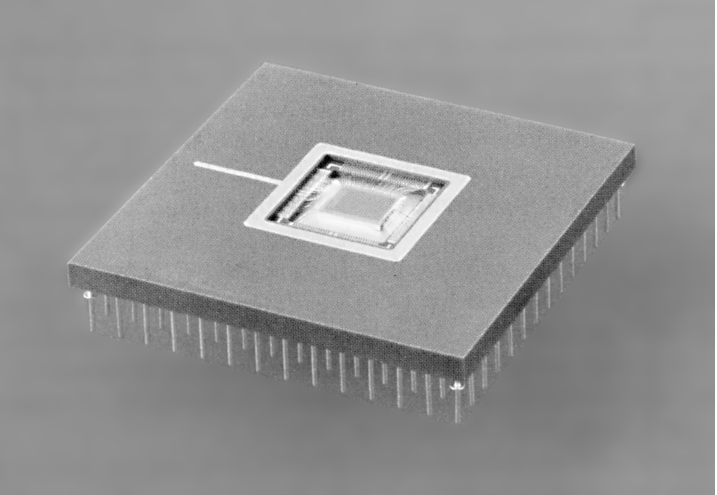
\includegraphics[width=0.8\textwidth]{scalony.png}
\centering
\caption{Sieć neuronowa zrealizowana w formie układu scalonego. Liczba neuronów samej sieci wynosi 16 x 16 = 256. Układ zawiera około 60 000 tranzystorów \citep[s. 14]{Kosinski2017} i \citep{Chua1998}.}
\centering
\end{center}
\end{figure}

Jak do tej pory sztuczne sieci neuronowe wykorzystywano do realizacji wielu skomplikowanych zadań. Jednym z najważniejszych zastosowań jest wykorzystanie sztucznych sieci neuronowych do rozpoznawania obiektów występujących na obrazie. Mogą być to obrazy różnego rodzaju - na przykład tę przedstawiające pismo odręczne (zob. rys 2). Sieci neuronowe są również szeroko wykorzystywane do rozwiązywania różnego rodzaju problemów optymalizacyjnych czy do przewidywania ruchów inwestorów na giełdzie \citep[s. 15]{Kosinski2017}.

\begin{figure}[H]
\begin{center}
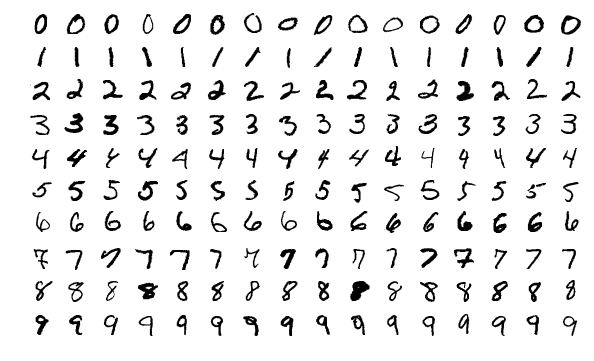
\includegraphics[width=\textwidth]{MINST.png}
\caption{Baza danych \textit{MNIST} zawiera skany odręcznych cyfr, które są powszechnie wykorzystywane w procesie uczenia różnych systemów przetwarzania obrazu. Źródło: \href{https://en.wikipedia.org/wiki/MNIST_database}{Wikipedia}}
\centering
\end{center}
\end{figure}

Sieci neuronowe -- zarówno te biologiczne jak ich sztuczne odpowiedniki -- są systemem złożonym. Mają one właściwości charakterystyczne dla sieci typu \textit{małego świata}. To znaczy, że najkrótsza droga $L$ między dwoma neuronami sieci jest stosunkowo krótka, a prawdopodobieństwo $P$ tego, że neuron ma $k$ sąsiednich neuronów, z którymi jest połączony jest wprost proporcjonalne do wartości $k^{-\Upsilon}$, gdzie stała wartość $2 < \Upsilon < 3$ -- zależy od architektury sieci neuronowej. Na rysunku 3 przedstawiono kilka przykładów takich architektur (Za: \citep[s. 15-16]{Kosinski2017}).

\begin{figure}[H]
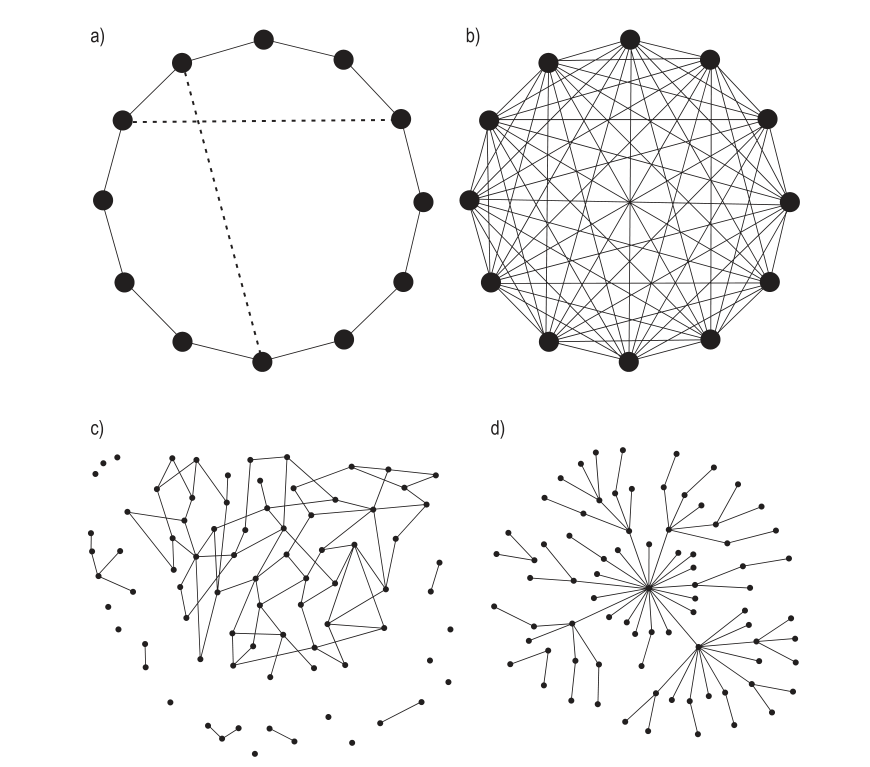
\includegraphics[width =\textwidth]{architektura.png}
\centering
\caption{(a) sieć jednowymiarowa z połączeniami bliskozasięgowymi (linie ciągłe) oraz z połączeniami typu \textit{małego swiata} (linie przerywane (b) sieć całkowicie połączona o 12 węzłach (c) sieć przypadkowo połączona (graf przypadkowy) (d) sieć bezskalowa\protect\footnotemark}
\centering
\end{figure}

\footnotetext{Sieć, w której rozkład liczby połączeń między węzłami jest zgodny z rozkładem \textit{Yule-Simona:}
P(k)\textasciitilde $k^{-\Upsilon}$. \\ gdzie $\Upsilon$ jest parametrem właściwym dla danej sieci i przyjmuje wartości z zakresu (2,3)  Źródło: \href{https://en.wikipedia.org/wiki/Scale-free_network}{Wikipedia}}

\clearpage
\section{Poznanie a rozpoznanie}
Problem automatycznego rozpoznawania obiektów będę tutaj rozpatrywać bazując na idei podziału przestrzeni wyników na rozłączne zbiory (klasy). Wyróżnione zbiory powinny określać wartości wyników obserwacji właściwe poszczególnym obiektom badanego zbioru. \textit{Wynik obserwacji} przedstawia zaobserwowane lub zmierzone wartości cech danego obiektu \citep[s. 7]{Kwiatkowski2007}.

Przez \textit{przestrzeń wyników obserwacji} rozumiemy to samo co pod przestrzenią cech obiektu. Wynik obserwacji stanowi formalnie punkt przestrzeni cech.\footnote{Zakładamy tutaj, że badany przez nas wzór obiekt jest reprezentowany poprzez wektor liczb zwany wartościami cech. Przestrzeń na płaszczyźnie która zawiera wektory cech badanego obiektu nazywamy właśnie przestrzenią cech.} \textit{Rozpoznanie obiektu} polega zatem na obserwacji (pomiarze wartości) cech obiektu i~sprawdzeniu do której klasy w przestrzeni cech zaobserwowany wynik należy. Taki sposób wnioskowania jest charakterystyczny dla zadania \textit{klasyfikacji} \citep[s. 7]{Kwiatkowski2007}.

Podstawowym problemem jest sposób, w jaki dokonamy tego podziału przestrzeni na podstawie dostępnych danych. Kluczem do uzyskania satysfakcjonujących wyników może być sformułowanie we właściwy sposób zadania aproksymacji. Dzięki temu możliwe staje się wykorzystanie metody najmniejszych kwadratów do rekurencyjnego uzyskiwania rozwiązań. Taki sposób postępowania leży u podstaw działania sztucznych sieci neuronowych. Na bazie tego typu sieci zadania poznawania (uczenia się) i rozpoznawania uzyskują naturalną interpretacje \citep[s. 7-8]{Kwiatkowski2007}.

Ujmując problem bardziej ściśle, poprzez rozpoznanie rozumiem wyróżnienie przedmiotu spośród innych występujących w analizowanym zbiorze obiektów. Poznanie zwykle oznacza zdobywanie wiedzy o czymś, nauczenie się czegoś na podstawie doświadczenia. Proces poznawania będę tutaj utożsamiać z uczeniem się.
Wyróżniamy dwa sposoby uczenia się:

\begin{enumerate}[leftmargin=2\parindent] % do wciecia
    \item Uczenie się z nauczycielem (nadzorowane),
    \item Uczenie się bez nauczyciela (nienadzorowane)
\end{enumerate}

Uczenie z nauczycielem polega na wstępnym określeniu cech charakterystycznych dla każdego badanego obiektu: nauczyciel przedstawia wynik obserwacji cech wraz z określeniem właściwego rodzaju obiektu (właściwego wyniku klasyfikacji obiektu). Nauczenie polega na określeniu w przestrzeni cech zbioru wartości właściwych danego obiektu. Rezultatem uczenia jest określenie podzbiorów przestrzeni cech charakteryzujących poszczególne obiekty \citep[s. 8]{Kwiatkowski2007}.

Sposób drugi polega na grupowaniu tych obserwacji, które powodują taką samą reakcje programu dokonującego klasyfikacji. Należy zaznaczyć, że nie zawsze dochodzi tutaj do znalezienia relacji przyczynowo-skutkowej -- często obserwacje są kojarzone w jedną grupę na podstawie innych, często nieintuicyjnych cech obiektów.
Jeśli wyróżnione podzbiory tworzą podział przestrzeni cech (tzn. są rozłączne i wyczerpują całą badaną przestrzeń), to dzięki uzyskaniu odpowiednich klas abstrakcji (grup) możemy zdefiniować nowe obiekty w taki sposób, że każda z dostępnych klas definiuje obiekt \citep[s. 8-9]{Kwiatkowski2007}.

\section{Model sztucznego neuronu}
Jednym z najprostszych modeli sieci neuronowych jest \textbf{sztuczny neuron}. Pojedyncze sztuczne neurony to modele obliczeniowe, które zapoczątkowały rozwój uczenia maszynowego \citep[s. 39]{Raschka_2019}.
Model sztucznego neuronu został zainspirowany -- jak nazwa wskazuje -- neuronem biologicznym, który został przedstawiony na rysunku 4.
\begin{figure}[H]
\begin{center}
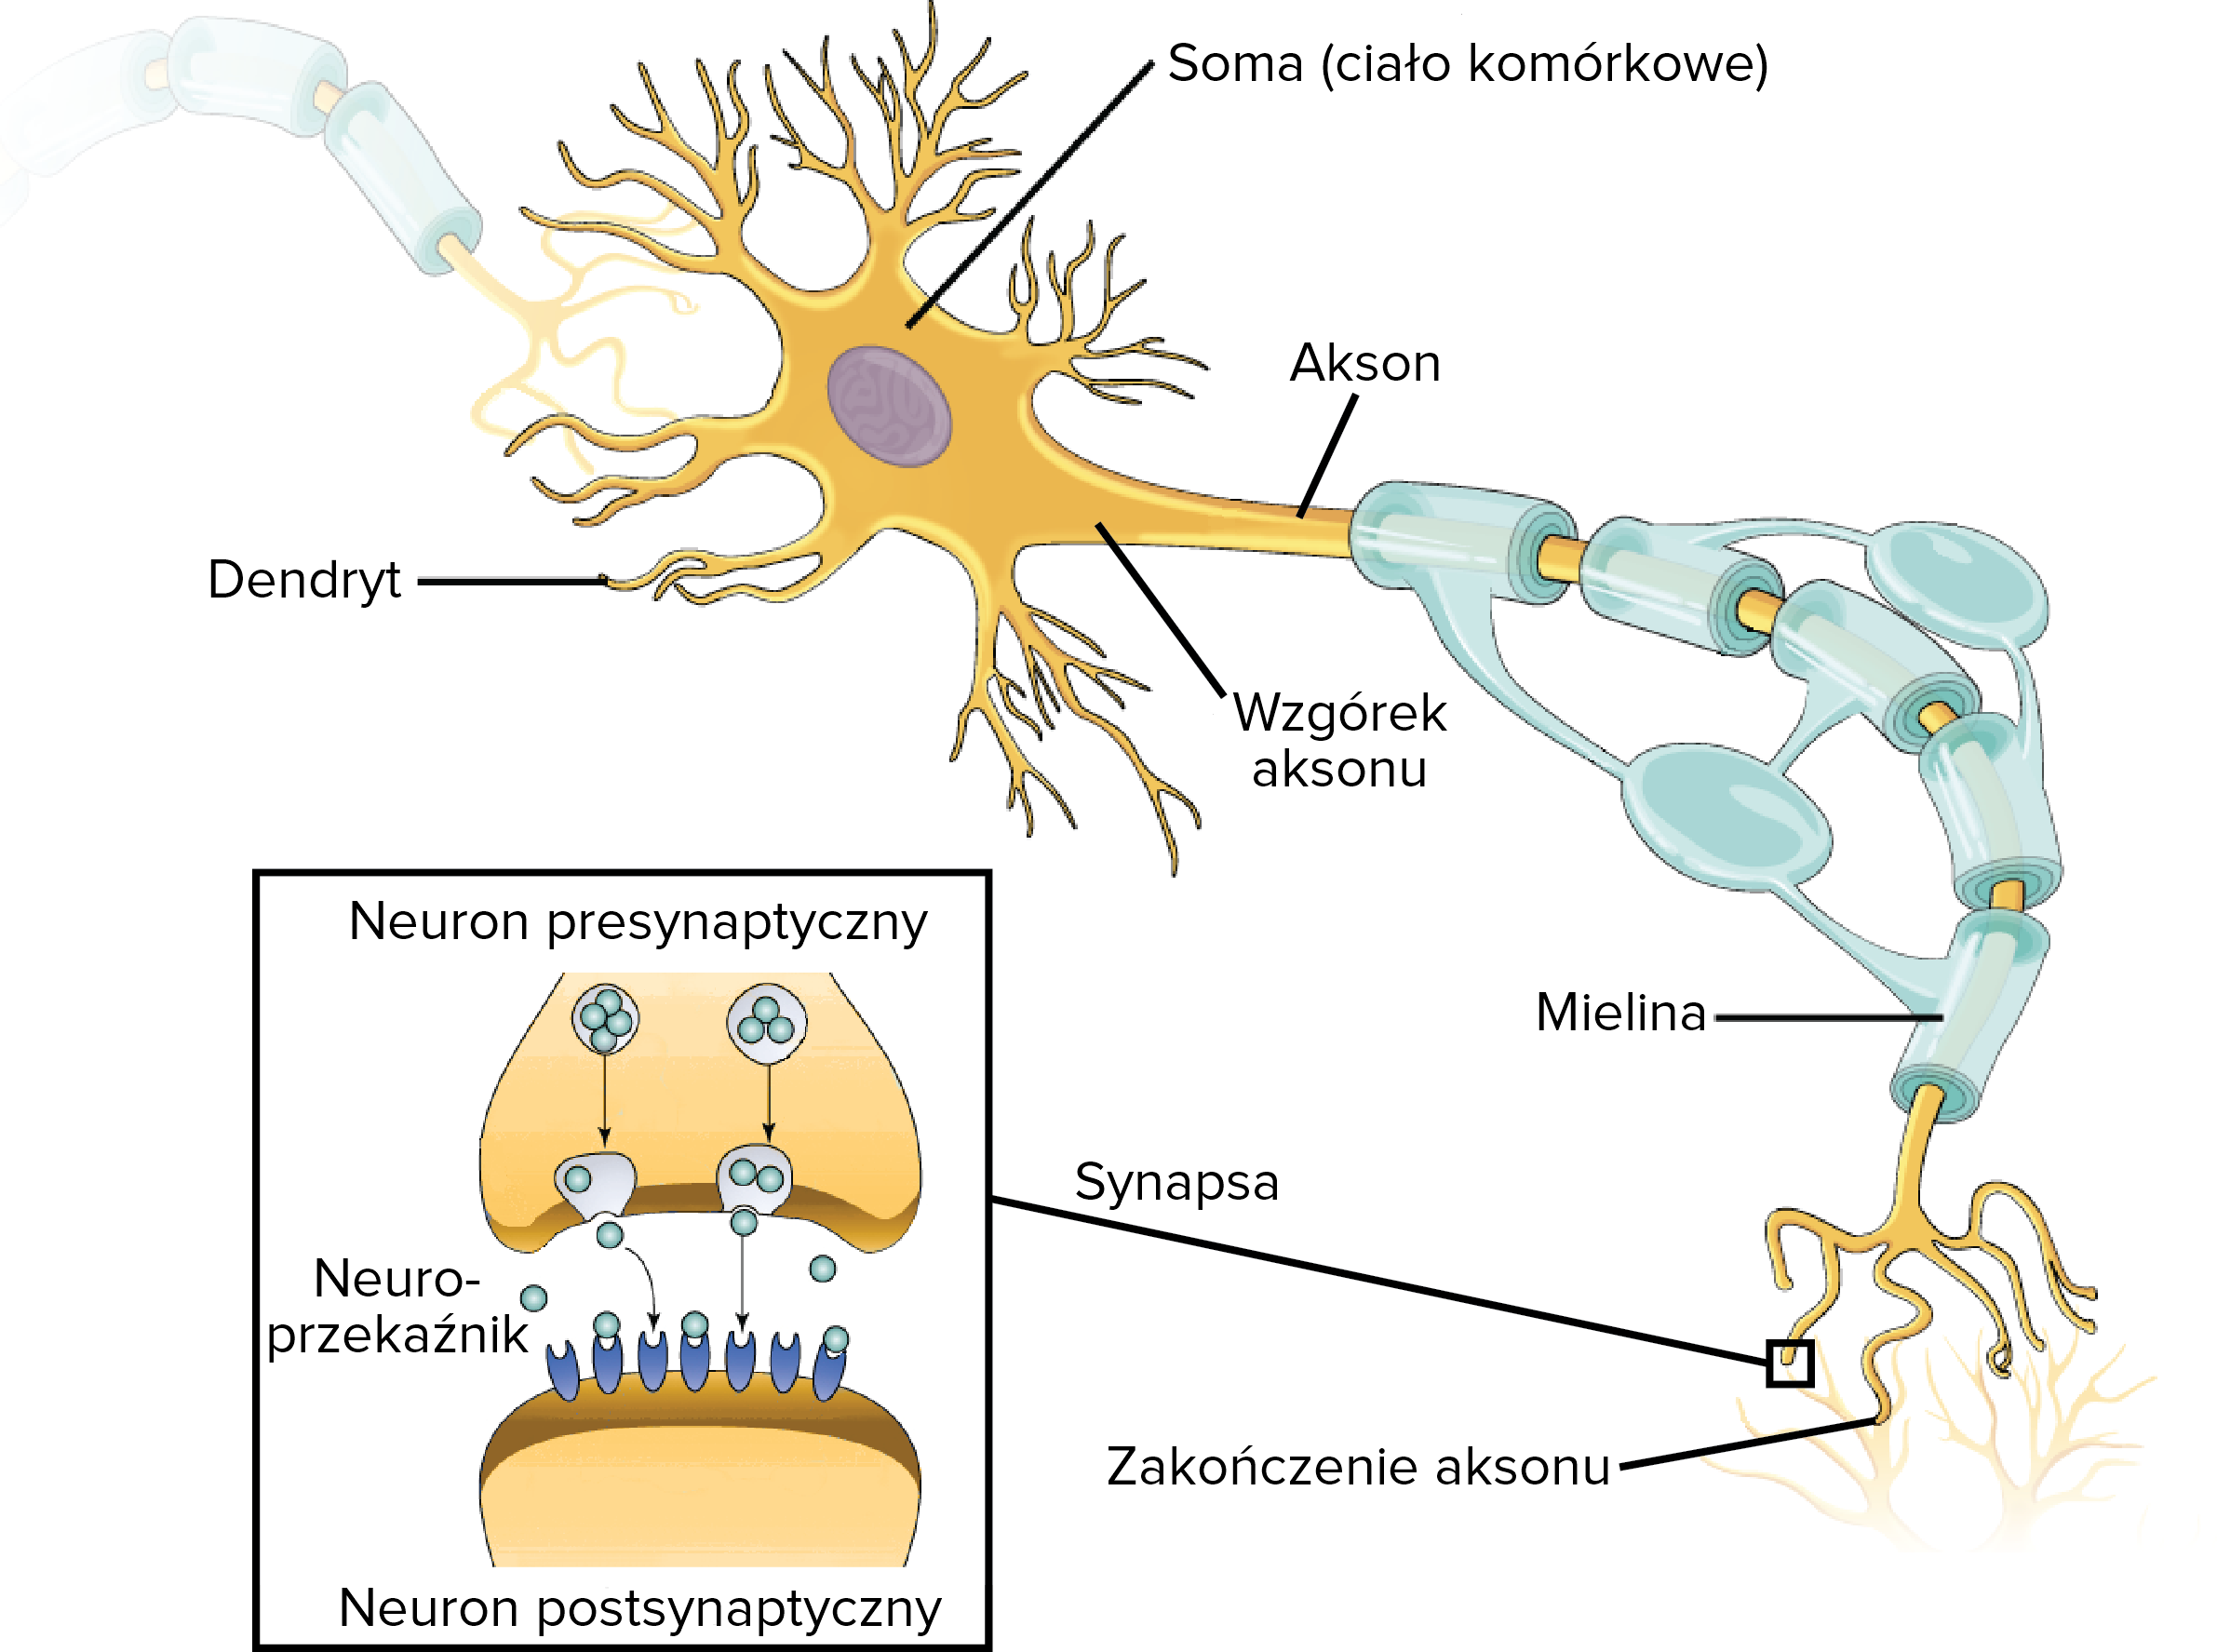
\includegraphics[width=0.8\textwidth]{neuron.png}
\caption{Model neuronu biologicznego. Źródło: \href{https://pl.khanacademy.org/science/biology/human-biology/neuron-nervous-system/a/overview-of-neuron-structure-and-function}{Khan Academy}}
\centering
\end{center}
\end{figure}

Jedną z pierwszych prób formalnego zdefiniowania zasady działania neuronu biologicznego podjeli w roku 1943 \textit{McCulloch} i \textit{Pitts}. Zaproponowali oni pierwszy model sztucznego neuronu tzw. \textbf{Neuron McCullocha-Pittsa} (zob. Rys. 5).

McCulloch i Pitts opisali neuron jako bramkę logiczną zawierającą binarne wyjścia. Zasada działania tego modelu jest prosta: do neuronu dociera wiele sygnałów, które po integracji w ciele komórki generują sygnał na wyjściu, jeżeli zostanie przekroczona odgórnie ustalona wartość graniczna. Jeśli coś takiego nie będzie miało miejsca -- neuron nie wygeneruje odpowiedzi na wyjściu \citep[s. 40]{Raschka_2019}.
\begin{figure}[H]
\begin{center}
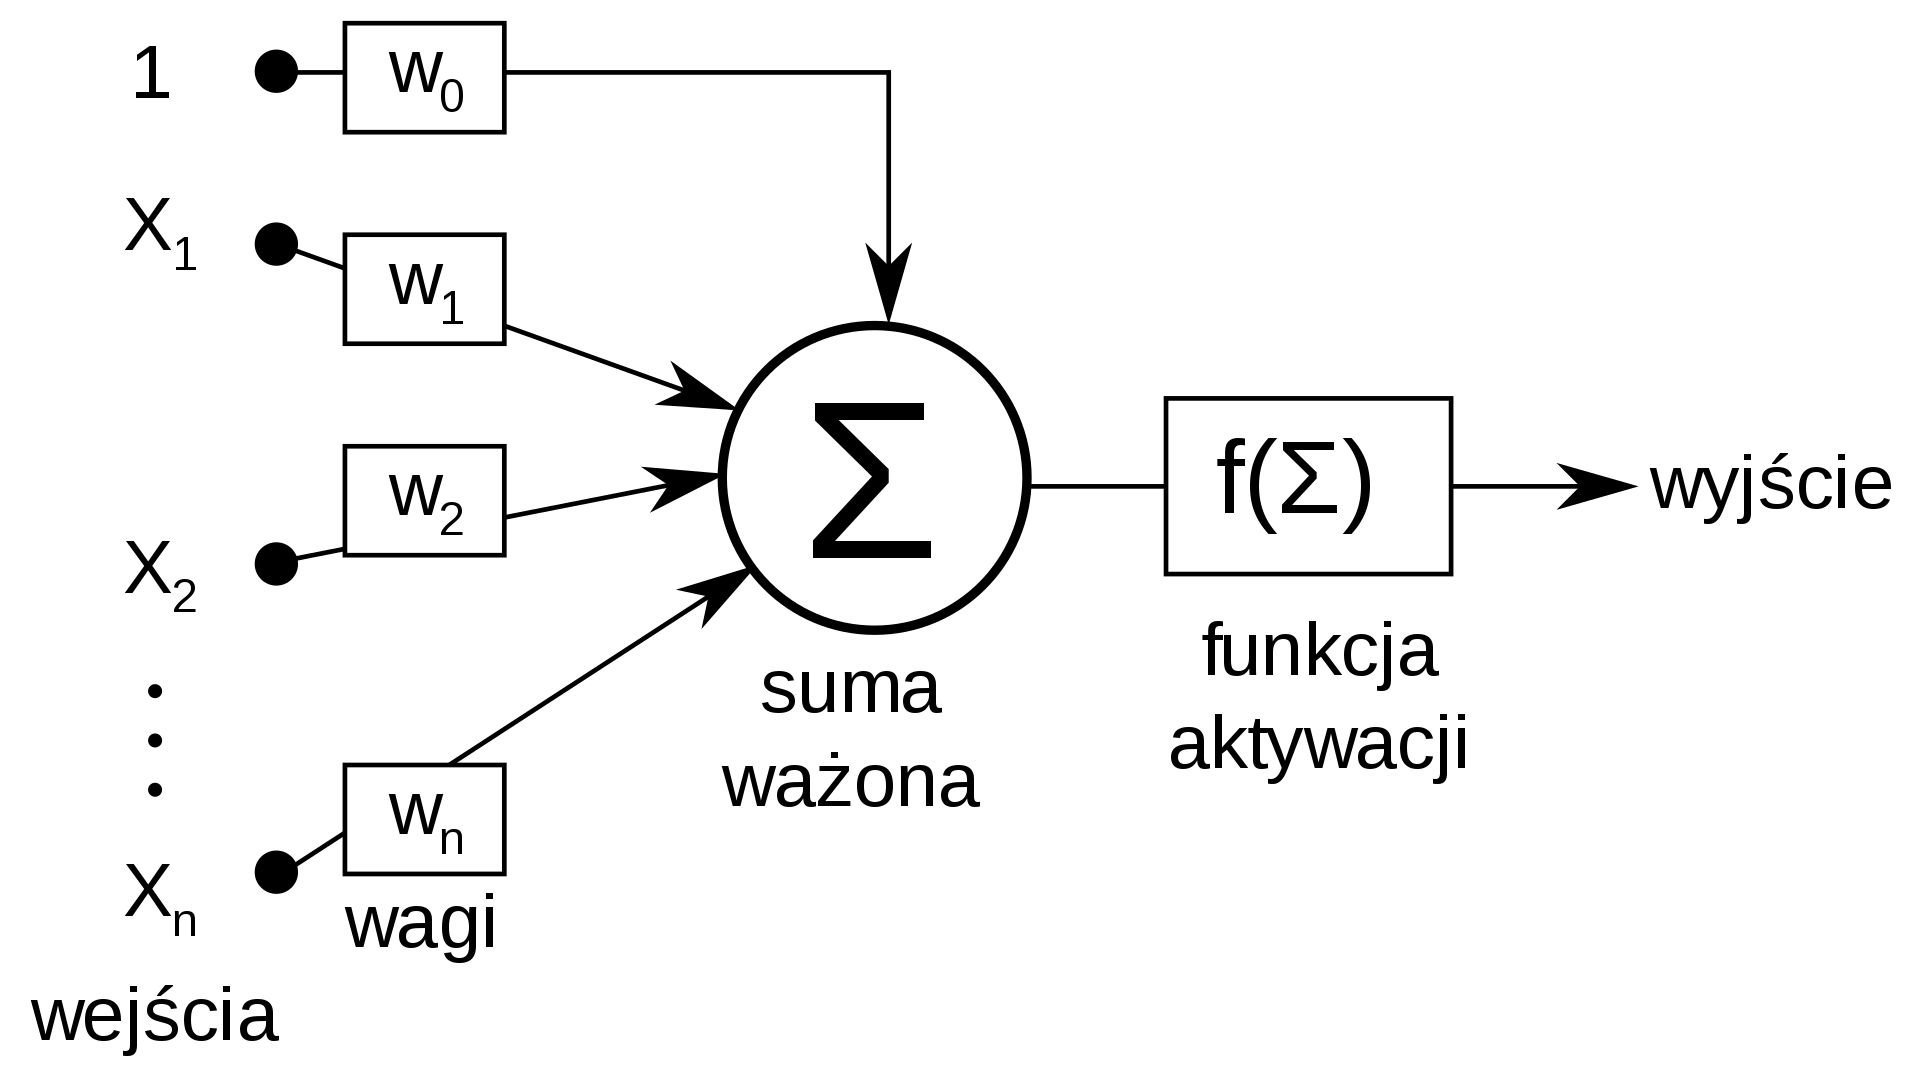
\includegraphics[width=0.8\textwidth]{Pitts.png}
\caption{Model neuronu McCullocha-Pittsa. Jeśli wartość sumy ważonej przekroczy wartośc progową funkcji aktywacji, to zostanie wygenerowana odpowiedź neuronu na wyjściu komórki. Źródło: \href{https://pl.wikipedia.org/wiki/Neuron_McCullocha-Pittsa}{Wikipedia}}
\centering
\end{center}
\end{figure}
Innym przykładem jest \textbf{Perceptron Rosenblatta}. Frank Rosenblatt zaproponował algorytm zdolny do automatycznego uczenia się za pomocą optymalnych współczynników wag, które są przemnażane przez wartości obecne na wejściu neuronu, co pozwala w jednoznaczny sposób określić czy neuron ma przekazać dalej otrzymany sygnał. W kontekście uczenia nadzorowanego można wykorzystać ten mechanizm do realizacji zadania klasyfikacji obiektu do różnych klas \citep[s.40]{Raschka_2019}.

\section{Cel pracy}

Celem pracy nie jest opis konkretnej implementacji sieci neuronowej ani zaprojektowanie takiej sieci od podstaw. Celem, który zamierzamy zrealizować w niniejszej pracy jest  zastosowanie pewnych cech i funkcji typowych dla sieci neuronowej do realizacji zadania kompozycji dzieła muzycznego. Sieć neuronowa jest mechanizmem opracowanym do rozpoznawania pewnych wzorców w danych i podejmowaniu na ich podstawie konkretnych decyzji lub tylko sugerowaniu pewnych rozwiązań właściwym decydentom. Te właściwość sieci zamierzamy właśnie wykorzystać. Planujemy zbudować system, który właściwie rozpozna cechy dzieła muzycznego i będzie w stanie je uogólnić do rozpoznawania ich  w szerszej klasie przykładów (zadanie klasyfikacji). Dodatkowo chcemy aby system dysponował zdolnością do tworzenia nowego utworu muzycznego na podstawie gotowego przykładu (zadanie generowania muzyki). Do realizacji tego zadania skorzystamy z pewnych cech, które zwyczajowo w literaturze przypisuje się właśnie sztucznym sieciom neuronowym.   
